\documentclass{article}
\usepackage{amsmath}
\usepackage{graphicx}
\usepackage{listings}
\usepackage{caption}
\usepackage{hyperref}

\title{License Plate Recognition Algorithm Explanation}
\author{}
\date{}

\begin{document}
	
	\maketitle
	
	\section{Image channel}
	In OpenCV, images can be represented as channels 1, 2, 3, and 4:
	\begin{itemize}
		\item Channel 1 is a grayscale image.
		\item 2-channel images include RGB555 and RGB565. RGB555 uses 16 bits (5+6+5) to store the color information, where 5 bits are for red, 6 bits for green, and 5 bits for blue. This is often used for program processing, like Fourier transforms, where one channel is real and the other is imaginary.
		\item 3-channel images are RGB color images.
		\item 4-channel images are RGBA, where A represents the alpha channel, or transparency. PNG images typically use 4 channels. The alpha channel can range from 0 to 255, representing full transparency to full opacity.
	\end{itemize}
	
	\textbf{CvType type constant combination rules:}
	\begin{itemize}
		\item \textbf{Byte:} Refers to the number of bits used. It can be 8, 16, 32, or 64 bits.
		\item \textbf{U|S|F:}
		\begin{itemize}
			\item U: Unsigned integer
			\item S: Signed integer
			\item F: Float (single precision)
		\end{itemize}
		\item \textbf{C [channels]:} The number of channels in the image.
	\end{itemize}
	\textbf{Example:} \texttt{CV\_8UC3} refers to an 8-bit unsigned, 3-channel (RGB color) image.
	
	\section{Grayscale Image}
	Color images usually have three components: R, G, and B. Grayscale conversion is the process of making the R, G, and B components equal for each pixel. Each pixel in a grayscale image has only one sample color, ranging from 0 (black) to 255 (white). Higher grayscale values are brighter, and lower values are darker.
	
	Grayscale conversion in OpenCV:
	\begin{verbatim}
		Imgproc.cvtColor(inMat, dst, Imgproc.COLOR_BGR2GRAY);
	\end{verbatim}
	
	\href{https://leejason.blog.csdn.net/article/details/106416128}{Source Link}
	
	\section{Image Filtering (Noise Reduction)}
	Image filtering reduces noise in the target image while preserving its detailed features. There are two types of filtering:
	\begin{itemize}
		\item Blurring
		\item Noise elimination
	\end{itemize}
	
	\subsection{Gaussian Filtering}
	Also known as Gaussian blur, it works by convolving the image with a Gaussian kernel (3x3, 5x5). This operation smooths the image and reduces noise. Gaussian filtering is better at preserving details than mean filtering.
	
	Example:
	\begin{verbatim}
		public static final int BLUR_KERNEL = 3;
		public static void gaussianBlur(Mat inMat, Mat dst) {
			Size ksize = new Size(BLUR_KERNEL, BLUR_KERNEL); // 3x3
			Imgproc.GaussianBlur(inMat, dst, ksize, 0, 0, Core.BORDER_DEFAULT);
		}
	\end{verbatim}
	
	\subsection{Median Filtering}
	Median filtering replaces the grayscale value of a pixel with the median value of its neighbors. It is very effective in removing speckle noise and salt-and-pepper noise.
	
	Example:
	\begin{verbatim}
		public static void medianBlur(Mat inMat, Mat dst) {
			Imgproc.medianBlur(inMat, dst, 3);
		}
	\end{verbatim}
	
	\subsection{Mean Filtering}
	Mean filtering averages the pixel values in a region. However, it can blur the image and reduce details, making it ineffective at removing noise like salt-and-pepper noise.
	
	Example:
	\begin{verbatim}
		public static void blur(Mat inMat, Mat dst) {
			Imgproc.blur(inMat, dst, new Size(5, 5));
		}
	\end{verbatim}
	
	\section{Affine Transformation}
	Affine transformations involve geometric operations like scaling, rotating, and translating an image. It includes:
	\begin{itemize}
		\item Transforming spatial coordinates
		\item Using interpolation to fill pixel values in the output image
	\end{itemize}
	
	Common interpolation methods:
	\begin{itemize}
		\item INTER\_NEAREST: Nearest neighbor interpolation
		\item INTER\_LINEAR: Bilinear interpolation (default)
		\item INTER\_AREA: Used for downsampling
		\item INTER\_CUBIC: Bicubic interpolation (4x4 pixel neighborhood)
		\item INTER\_LANCZOS4: Lanczos interpolation (8x8 pixel neighborhood)
	\end{itemize}
	
	\subsection{Translation}
	Translation is the simplest affine transformation, moving the image along the x and y axes.
	
	\begin{equation}
		\text{dst} = A \times \text{inMat}
	\end{equation}
	where $A$ is the affine transformation matrix.
	
	Example:
	\begin{verbatim}
		public static void translateImg(Mat inMat, Mat dst, int pX, int pY) {
			Mat trans_mat = Mat.zeros(2, 3, CvType.CV_32FC1);
			trans_mat.put(0, 0, 1);
			trans_mat.put(0, 2, pX);
			trans_mat.put(1, 1, 1);
			trans_mat.put(1, 2, pY);
			Imgproc.warpAffine(inMat, dst, trans_mat, inMat.size());
		}
	\end{verbatim}
	
	\subsection{Scaling}
	Scaling changes the size of the image by applying a transformation matrix. To avoid image distortion, the aspect ratio should be locked.
	
	Example:
	\begin{verbatim}
		public static Mat zoom(Mat inMat, Integer maxWidth) {
			double ratio = maxWidth * 1.0 / inMat.width();
			Integer maxHeight = (int) Math.round(ratio * inMat.height());
			Mat dst = new Mat(maxHeight, maxWidth, inMat.type());
			Imgproc.resize(inMat, dst, dst.size(), ratio, ratio, Imgproc.INTER_CUBIC);
			return dst;
		}
	\end{verbatim}
	
	\subsection{Rotation}
	Rotation involves rotating the image by a specified angle. Positive angles result in clockwise rotation, while negative angles result in counterclockwise rotation.
	
	Example:
	\begin{verbatim}
		public static void rotateImg(Mat inMat, Mat dst, double angle, Point center) {
			Mat img_rotated = Imgproc.getRotationMatrix2D(center, angle, 1);
			Imgproc.warpAffine(inMat, dst, img_rotated, inMat.size());
		}
	\end{verbatim}
	
	\subsection{Affine Transformation (Skew Correction)}
	Affine transformation can correct image skew by taking three points from the original image and calculating the transformation matrix.
	
	Example:
	\begin{verbatim}
		public static void warpAffine(Mat inMat, Mat dst) {
			MatOfPoint2f srcPoints = new MatOfPoint2f();
			srcPoints.fromArray(new Point(0, 0), new Point(0, inMat.rows()), 
			new Point(inMat.cols(), 0));
			MatOfPoint2f dstPoints = new MatOfPoint2f();
			dstPoints.fromArray(new Point(80, 0), new Point(-80, inMat.rows()), 
			new Point(inMat.cols() + 80, 0));
			Mat trans_mat = Imgproc.getAffineTransform(srcPoints, dstPoints);
			Imgproc.warpAffine(inMat, dst, trans_mat, inMat.size());
		}
	\end{verbatim}
	
	\subsection{Projection Transformation}
	Projection transformation maps an image onto a new plane. It is similar to projecting a movie onto a screen.
	
	Example:
	\begin{verbatim}
		public static void warpPerspective(Mat inMat, Mat dst) {
			MatOfPoint2f srcPoints = new MatOfPoint2f();
			srcPoints.fromArray(new Point(0, 0), new Point(0, inMat.rows()), 
			new Point(inMat.cols(), 0), new Point(inMat.cols(), inMat.rows()));
			MatOfPoint2f dstPoints = new MatOfPoint2f();
			dstPoints.fromArray(new Point(80, 0), new Point(-80, inMat.rows()), 
			new Point(inMat.cols() + 80, 0), new Point(inMat.cols() - 80, inMat.rows()));
			Mat trans_mat = Imgproc.getPerspectiveTransform(srcPoints, dstPoints);
			Imgproc.warpPerspective(inMat, dst, trans_mat, inMat.size());
		}
	\end{verbatim}
	
	\section{Edge Detection}
	\begin{figure}[h]
		\centering
		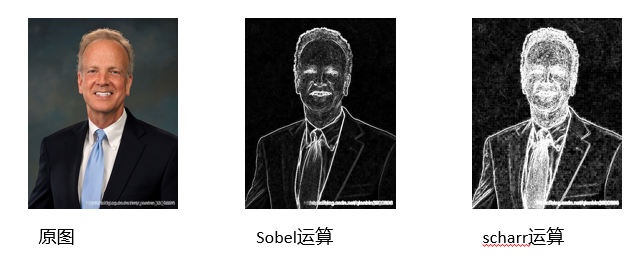
\includegraphics[width=0.5\textwidth]{mdpic/20240919165105.png}
		\caption{Edge detection example}
	\end{figure}
	
	\subsection{Sobel Operator}
	The Sobel operator is a first-order gradient algorithm that calculates the horizontal and vertical derivatives of an image, highlighting edges.
	
	Example:
	\begin{verbatim}
		public static final int SOBEL_SCALE = 1;
		publicstatic final int SOBEL_DELTA = 0;
		public static final int SOBEL_DDEPTH = CvType.CV_16S;
		public static void sobel(Mat inMat, Mat dst) {
			Mat gradX = new Mat(), gradY = new Mat();
			Mat absGradX = new Mat(), absGradY = new Mat();
			
			// Calculate gradients in X and Y direction
			Imgproc.Sobel(inMat, gradX, SOBEL_DDEPTH, 1, 0, 3, SOBEL_SCALE, SOBEL_DELTA, Core.BORDER_DEFAULT);
			Imgproc.Sobel(inMat, gradY, SOBEL_DDEPTH, 0, 1, 3, SOBEL_SCALE, SOBEL_DELTA, Core.BORDER_DEFAULT);
			
			// Convert gradients to absolute value
			Core.convertScaleAbs(gradX, absGradX);
			Core.convertScaleAbs(gradY, absGradY);
			
			// Combine gradients
			Core.addWeighted(absGradX, 0.5, absGradY, 0.5, 0, dst);
		}
		\end{verbatim}
		
		\subsection{Canny Edge Detection}
		The Canny edge detection algorithm involves the following steps:
		\begin{enumerate}
		\item Use Gaussian blur to remove noise.
		\item Compute gradients using Sobel operator.
		\item Use non-maximum suppression to eliminate false edges.
		\item Apply double threshold to detect strong and weak edges.
		\item Track edges by hysteresis to form continuous edges.
		\end{enumerate}
		
		Example:
		\begin{verbatim}
		public static void canny(Mat inMat, Mat dst, double threshold1, double threshold2) {
			Imgproc.Canny(inMat, dst, threshold1, threshold2);
		}
		\end{verbatim}
		
		\section{License Plate Recognition Example}
		\begin{enumerate}
		\item Load the image.
		\item Convert the image to grayscale.
		\item Use Gaussian blur to reduce noise.
		\item Apply Sobel operator to extract horizontal edges.
		\item Apply binary threshold to emphasize the edges.
		\item Use morphological operations to highlight potential regions of interest.
		\item Perform contour detection and filter by aspect ratio and size to isolate the license plate.
		\item Apply perspective transformation to straighten the license plate.
		\item Use Optical Character Recognition (OCR) to read the license plate text.
		\end{enumerate}
		
		Example code:
		\begin{verbatim}
		public static void recognizeLicensePlate(Mat inMat) {
			// Step 1: Convert to grayscale
			Mat gray = new Mat();
			Imgproc.cvtColor(inMat, gray, Imgproc.COLOR_BGR2GRAY);
			
			// Step 2: Apply Gaussian blur
			Mat blurred = new Mat();
			Imgproc.GaussianBlur(gray, blurred, new Size(5, 5), 0);
			
			// Step 3: Sobel operator to find edges
			Mat sobel = new Mat();
			sobel(blurred, sobel);
			
			// Step 4: Apply binary threshold
			Mat binary = new Mat();
			Imgproc.threshold(sobel, binary, 0, 255, Imgproc.THRESH_BINARY + Imgproc.THRESH_OTSU);
			
			// Step 5: Morphological operations (dilation and erosion)
			Mat morph = new Mat();
			Mat element = Imgproc.getStructuringElement(Imgproc.MORPH_RECT, new Size(17, 3));
			Imgproc.morphologyEx(binary, morph, Imgproc.MORPH_CLOSE, element);
			
			// Step 6: Find contours
			List<MatOfPoint> contours = new ArrayList<>();
			Mat hierarchy = new Mat();
			Imgproc.findContours(morph, contours, hierarchy, Imgproc.RETR_EXTERNAL, Imgproc.CHAIN_APPROX_SIMPLE);
			
			// Step 7: Filter contours by size and aspect ratio
			for (MatOfPoint contour : contours) {
				Rect rect = Imgproc.boundingRect(contour);
				if (isPlateSize(rect)) {
					Mat plate = new Mat(inMat, rect);
					
					// Step 8: Perspective transformation (optional)
					Mat straightenedPlate = correctSkew(plate);
					
					// Step 9: OCR (Optical Character Recognition)
					String plateText = readText(straightenedPlate);
					System.out.println("License Plate: " + plateText);
				}
			}
		}
		\end{verbatim}
		
	\end{document}